\documentclass{article}

\usepackage{phdstyle}
\usepackage[numbers]{natbib}

\begin{document}

\section{Perturbation of the spin motion}
The spin precession axis of a particle involved in betatron motion precesses about the stable invariant spin axis defined on the closed orbit (CO).

This precession can be observed in polarization data as a rapid, small-amplitude oscillation (example in Figure~\ref{fig:Py_fit_residual_cut}) on top of the \emph{major effect} oscillation caused by the precession of spin about the CO axis. The frequency of this latter oscillation is used in the FD methodology as the EDM observable. It is estimated by fitting polarimetry data by a sine function. The rapid oscillations, therefore, constitute a model error.\footnote{A more sophisticated, for example autoregressive, model would solve this problem; however at a cost to precision.}

This model error will introduce a bias into the frequency estimate (the amplitude growth of the blue line oscillation in Figure~\ref{fig:Py_fit_residual_full} is due to the bias). In the following we investigate how this bias changes depending on the beam revolution direction, its stability over time, and the EDM estimate error introduced by it.

\subsection{Simulation: Uniform beam}
For simulation, we used an imperfect FS lattice, with E+B elements randomly tilted about the optical axis by angles picked from the normal distribution $N(4\cdot 10^{-3}, 5\cdot10^{-4})$ [rad]. The systematic $\avg{\Theta_{tilt}} = 4\cdot 10^{-3}$ radians was selected to ensure a sufficiently high radial precession rate, and hence reduce tracking time requirements. Tilts are simulated by applying a rotation matrix to the spin transfer map of the lattice as discussed in Section~\ref{sec:FakeSignalSimulation}. By doing it this way, we do not affect the orbital transfer map; that is, the closed orbit remains unchanged.

The beam was represented by an ensemble $E$ of 4,000 rays, split into four groups of 1,000 rays:
\begin{inparaenum}[1)]
\item rays offset from the CO at injection time in the $x$ coordinate,
\item in the $y$ cooridnate,
\item in both $x$ and $y$,
\item in $d := \sfrac{\Delta K}{K_0}$.
\end{inparaenum}
The $x$ and $y$ coordunates were uniformly sampled in the range $\pm 1$ mm, $d$ in the range $\pm 10^{-4}$. The reference energy $K_0 = 270.0092$ MeV (Frozen Spin energy for this lattice).

The beam polarization was computed from spin tracking data as
\[
\vec P = \frac{\sum_{i\in E} \vec s_i}{||\sum_{i\in E} \vec s_i||}.
\]

Then the vertical polarization component was fitted with the fit function $f = \sin(2\pi\cdot f \cdot t)$, with $f$ the only fitted parameter. This procedure was carried out for the (identical at injection) CW and CCW revolving beams. We also estimated the reference rays' (CW \& CCW) precession frequencies in the same way, by fitting the vertical spin component $S_y^{CO}$ of the reference particle. The fit results are presented in Table~\ref{tbl:FreqFit}. From this table, one can see that the polarization estimate is clearly biased toward the reference ray's estimate; however, the CW vs CCW estimates of either the reference ray or the polarization are statistically indistinguishable (assuming a normal distribution of the estimates, the hypothesis test for equality gives p-values of 30\% and higher). 

\begin{figure}[!h]
  \centering
  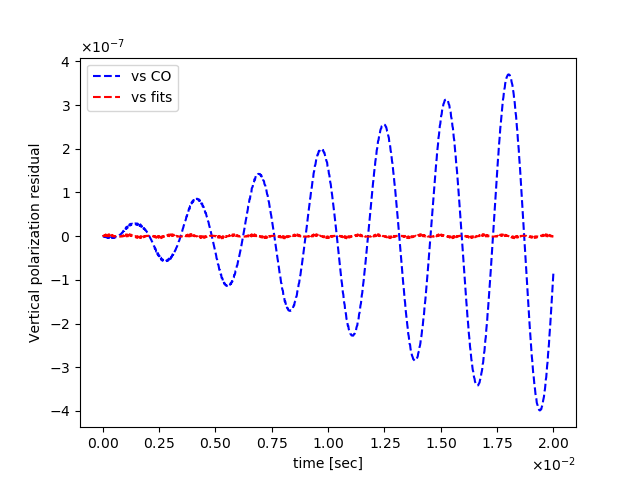
\includegraphics[width=\linewidth]{img/spin_axis_motion/long/CW_LONG_double_res_full}
  \caption{Vertical polarization residuals, computed as the difference between $P_y$ (data) and: (red) $\hat P_y$ (model prediction), (blue) $S_y^{co}$ (reference particle vertical spin component). The oscillations of the residuals are due to the rapid oscillations caused by the precession axis instability.\label{fig:Py_fit_residual_full}}
\end{figure}
\begin{figure}[!h]
  \centering
  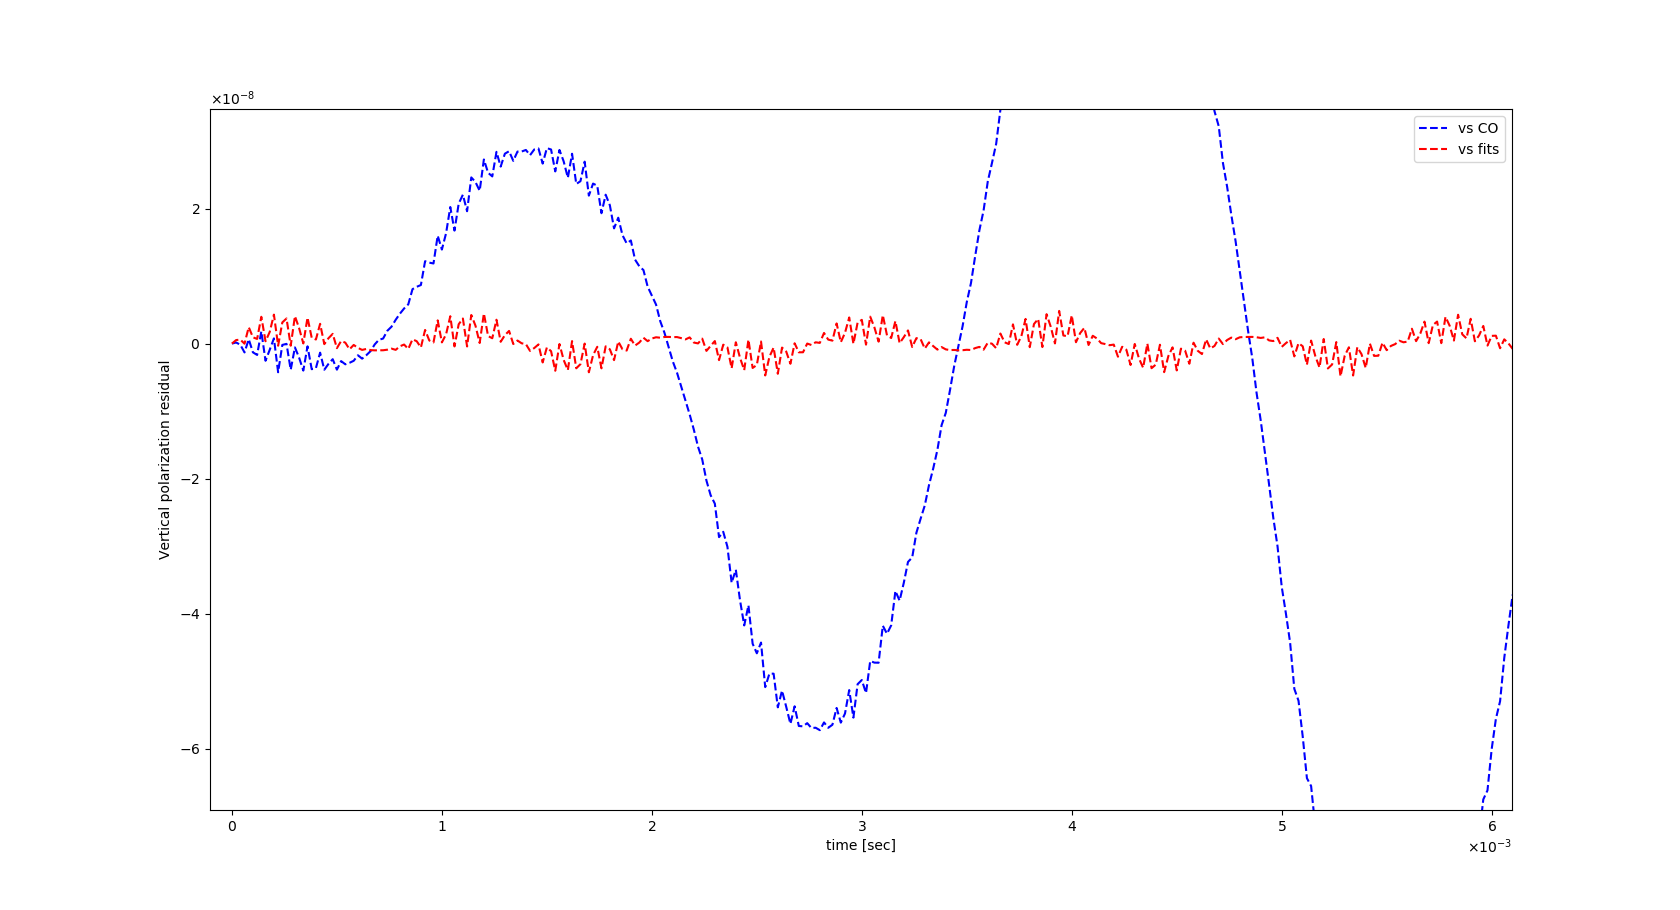
\includegraphics[width=\linewidth]{img/spin_axis_motion/long/CW_LONG_double_res_cut}
  \caption{A zoom of Figure~\ref{fig:Py_fit_residual_full}.\label{fig:Py_fit_residual_cut}}
\end{figure}

\begin{table}[!h]
  \centering
  \caption{Frequency estimates for the Uniform CW \& CCW beams, reference ray and full beam, in Hz\label{tbl:FreqFit}}
  \begin{tabular}{lc|rr|rr}
    \hline
    \multicolumn{2}{c}{Data}  & \multicolumn{2}{|c|}{Polarization} & \multicolumn{2}{|c}{Reference ray} \\
    \hline
      Frequency & Offset & CW  & CCW & CW & CCW \\
    \hline
    Estimate & 360.90365 & $1.58\cdot 10^{-7}$ & $1.57\cdot 10^{-7}$ & $3.42902\cdot 10^{-6}$ & $3.42902\cdot 10^{-6}$ \\
    SE & -- & $1\cdot 10^{-9}$& $2\cdot 10^{-9}$ & $5\cdot 10^{-10}$ & $5\cdot 10^{-10}$\\
    \hline
  \end{tabular}
\end{table}

%% As a last step, we conducted a moving frame fit of polarization data, in order to assess whether the model error might cause the frequency estimate to vary over time. The results are presented in Figure~\ref{fig:MovingFrameEstimates}.

%% \begin{figure}[!h] %% THIS PLOT NEEDS CHANGE OR REMOVAL !!!
%%   \centering
%%   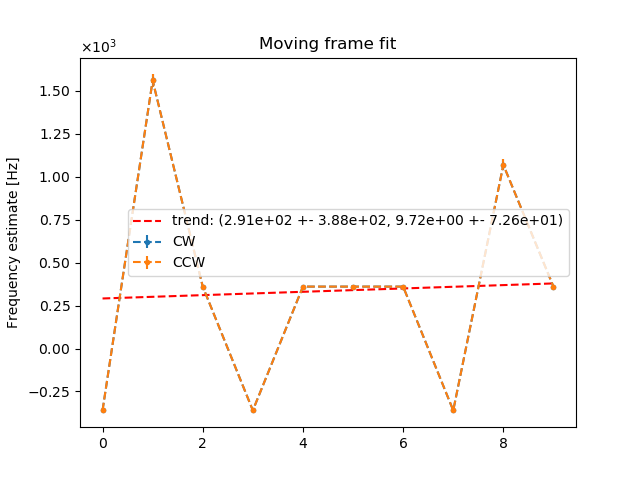
\includegraphics[width=\linewidth]{img/spin_axis_motion/long/moving_frame_freqs}
%%   \caption{Moving frame frequency estimates.\label{fig:MovingFrameEstimates}}
%% \end{figure}

\subsection{Simulation: Gaussian distribution beam}
For this test we injected a beam of the same size, with $x$, $y$ and $d$ coordinates distributed normally (with standard deviations 1 mm, 1 mm, and $10^{-4}$ respectively). The coordinate distributions of the CW \& CCW beams are presented in Figures~\ref{fig:Gauss_hists_XY} and~\ref{fig:Gauss_hists_D}. As one can see, the beam's centroids are split by $0.004$ mm in the horizontal direction, and $0.014$ mm in the vertical direction. This split will have an effect on the resultant frequency estimate bias difference.

\begin{figure}[!h]
  \centering
  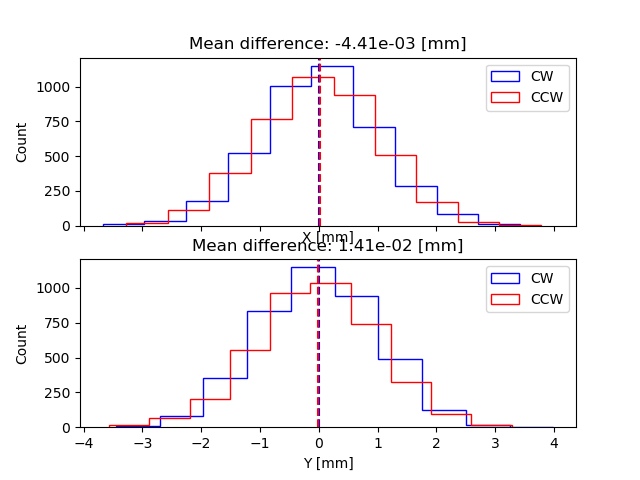
\includegraphics[width=\linewidth]{img/spin_axis_motion/presentation/beam_histograms_XY}
  \caption{The $x$ and $y$ initial beam distributions.\label{fig:Gauss_hists_XY}}
\end{figure}
\begin{figure}[!h]
  \centering
  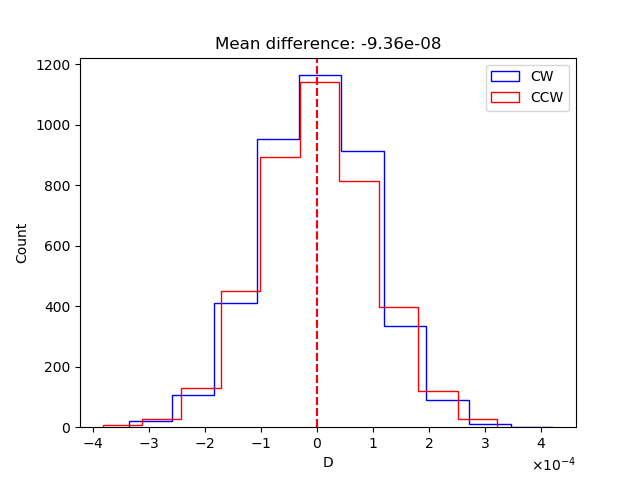
\includegraphics[width=\linewidth]{img/spin_axis_motion/presentation/beam_histograms_D}
  \caption{The $d$ initial beam distributions.\label{fig:Gauss_hists_D}}
\end{figure}

The fit results are summarized in Table~\ref{tbl:GaussBeamFreqFit}.

\begin{table}[!h]
  \centering
  \caption{Frequency estimates for the Gaussian CW \& CCW beams, reference ray and full beam, in Hz\label{tbl:GaussBeamFreqFit}}
  \begin{tabular}{lc|rr|rr}
    \hline
    \multicolumn{2}{c}{Data}  & \multicolumn{2}{|c|}{Polarization} & \multicolumn{2}{|c}{Reference ray} \\
    \hline
      Frequency & Offset & CW  & CCW & CW & CCW \\
    \hline
    Estimate & 352.99403 & $9.0405\cdot 10^{-6}$ & $7.792\cdot 10^{-6}$ & $4.149017\cdot 10^{-5}$ & $4.149017\cdot 10^{-5}$ \\
    SE & -- & $7\cdot 10^{-10}$& $9\cdot 10^{-9}$ & $2\cdot 10^{-11}$ & $2\cdot 10^{-11}$\\
    \hline
  \end{tabular}
\end{table}

The polarization frequency estimate difference 
\[
\varepsilon := \hat f_{CW} - \hat f_{CCW} = 1.249\cdot 10^{-6} \pm 9\cdot 10^{-9}~\text{[Hz]}.
\]
One can see that the difference cannot be explained by statistical uncertainty.

Together with the uniform beam simulation, the above result drives the conclusion that the beam distribution asymmetry is a source of systematic error via spin precession axis direction variation. This systematic effect should reduce with the beam size, as in that case the coordinate distributions become more symmetrical.

Considering the last point, assume $\varepsilon$ is proportional to the beam distribution centroid difference, defined by the coordinate distribution means. The expectation values of the coordinate distributions are located on the closed orbit, which is the same for the CW and CCW beams. The actual beam centroids are distributed about this point in a normal distribution with some standard deviation. Denote that standard deviation $\sigma_{mean} \equiv \sigma_{4k}$ for the beams used in the simulation above. This standard deviation gives us a frequency estimate variation on the order of $10^{-6}$ Hz (while the statistical uncertainty standard deviation is $10^{-9}$ Hz). The standard error of the mean is computed as
\[
\sigma_{mean} = \frac{\sigma}{\sqrt{n}},
\]
where $n$ is the sample size, which in our case is the number of beam particles.

Now, if we used a $n = 4\cdot10^{9}$ particle beam instead of the $n = 4\cdot10^{3}$ one, we'd have $\sigma_{4b} = \sigma_{4k}\cdot10^{-3}$. Assuming a linear relationship between the centroid difference and the frequency bias difference, the latter's standard deviation would reduce to $10^{-9}$, which is then comparable with statistical error.

\subsection{The effect of the beam distribution centroid difference on spin precession}

Now we will test the hypothesis that the estimate bias difference is proportional to the beam centroid difference. 

This time we repeated the test from the previous section for multiple (30) trials. We used the same imperfect lattice on each trial; trials only differ by their initial beam distributions. An example of the polarization oscillations in this lattice is given in Figure~\ref{fig:OscEx}.

\begin{figure}[!h]
  \centering
  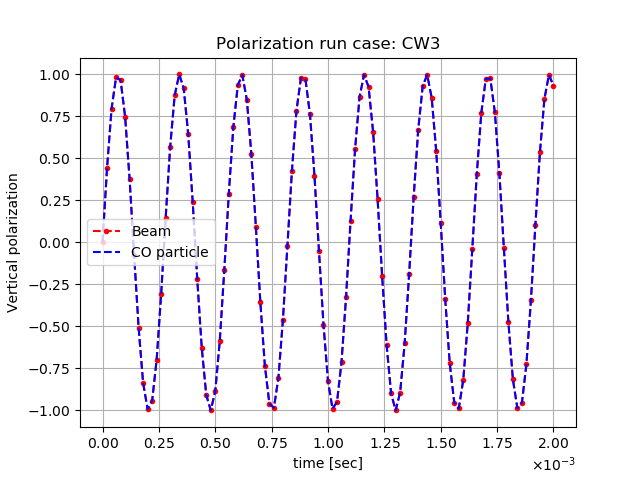
\includegraphics[width=\linewidth]{img/spin_axis_motion/multiple/CW3_polarization}
  \caption{Example of polarization oscillations in the used lattice.\label{fig:OscEx}}
\end{figure}


For each beam, we computed its centroid, defined as $\vec c = (\avg{x_0}, \avg{y_0}, \avg{d_0})$, and took the difference $\Delta\vec c := \vec c^{CW}_i - \vec c^{CCW}_i$ ($i$ the trial number). We then regressed (non-weighted linear regression) $\varepsilon_i$ on the components of $\Delta\vec c_i$. The results are plotted in Figure~\ref{fig:BiasVsCentroid}. We found a statistically significant dependence on the vertical centroid difference component (p-value $\approx 0$\%).

In order to make sure that the bias difference is not related to the change of the beam revolution direction, we checked the centroid difference dependence of the bias on the same direction beams. The dependence remains.

\begin{figure}[!h]
  \centering
  \begin{subfigure}[b]{\linewidth}
    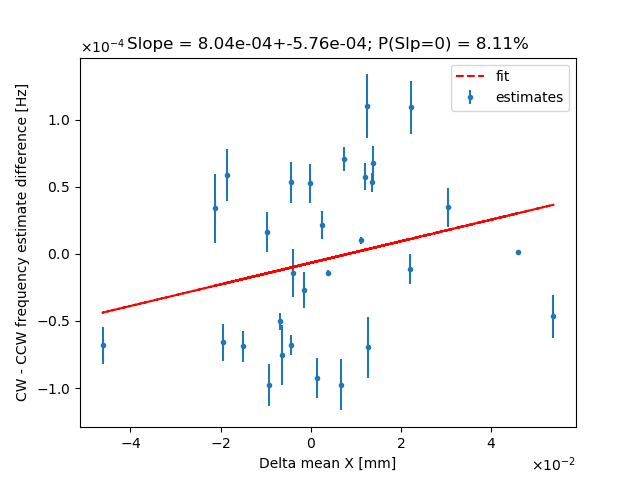
\includegraphics[width=\linewidth]{img/spin_axis_motion/multiple/freq_estimates_vs_centroid_diff_X}
    \caption{The $x$ coordinate.}
  \end{subfigure}
  \begin{subfigure}[b]{\linewidth}
    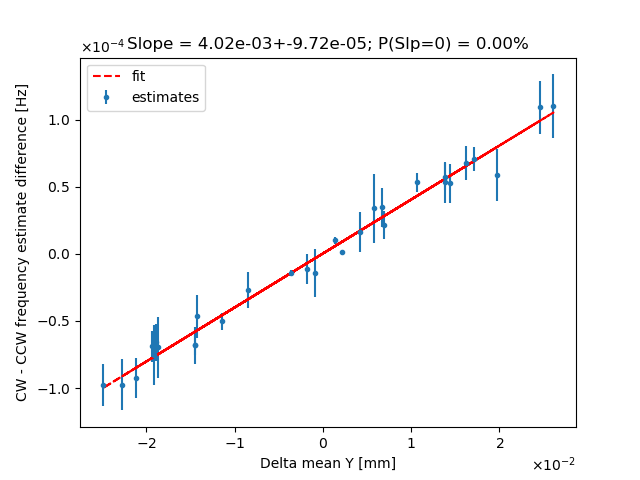
\includegraphics[width=\linewidth]{img/spin_axis_motion/multiple/freq_estimates_vs_centroid_diff_Y}
    \caption{The $y$ coordinate.}
  \end{subfigure}
\end{figure}
\begin{figure}[!h]\ContinuedFloat
  \centering
  \begin{subfigure}[b]{\linewidth}
    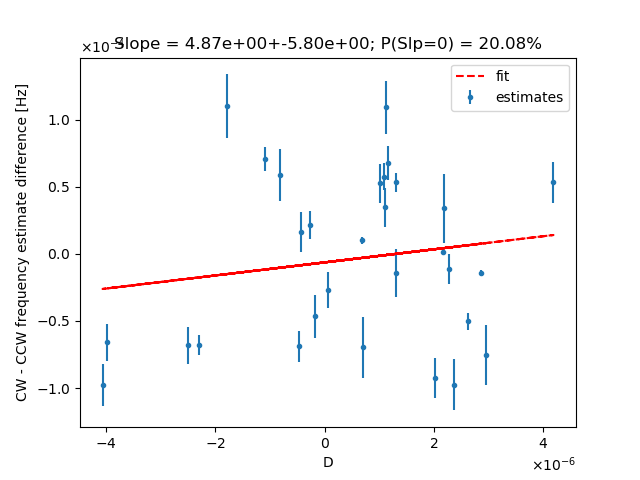
\includegraphics[width=\linewidth]{img/spin_axis_motion/multiple/freq_estimates_vs_centroid_diff_D}
    \caption{The $d$ coordinate.}
  \end{subfigure}
  \caption{Frequency estimate difference vs a beam centroid split coordinate.\label{fig:BiasVsCentroid}}
\end{figure}
 
\bibliography{PhDRefs}
\bibliographystyle{vancouver}


\end{document}

